\documentclass[11pt]{article}
\usepackage[utf8]{inputenc}
\usepackage[T1]{fontenc}
\usepackage{grffile}
\usepackage{longtable}
\usepackage{wrapfig}
\usepackage{rotating}
\usepackage[normalem]{ulem}
\usepackage{amsmath}
\usepackage{textcomp}
\usepackage{amssymb}
\usepackage{capt-of}
\usepackage{hyperref}
\hypersetup{colorlinks=true, linkcolor=magenta}
\setlength{\parindent}{0in}
\usepackage[margin=1in]{geometry}
\usepackage[english]{babel}
\usepackage{mathtools}
\usepackage{palatino}
\usepackage{fancyhdr}
\usepackage{sectsty}
\usepackage{engord}
\usepackage{parskip}
\usepackage{minted}
\usepackage{cite}
\usepackage{graphicx}
\usepackage{subcaption}
\usepackage{setspace}
\usepackage[compact]{titlesec}
\usepackage[center]{caption}
\usepackage{placeins}
\usepackage{color}
\usepackage{amsmath}
\usepackage{bm}
\usepackage{todonotes}
\usepackage{pdfpages}
% \titlespacing*{\subsection}{0pt}{5.5ex}{3.3ex}
% \titlespacing*{\section}{0pt}{5.5ex}{1ex}
\author{Luis Antonio Ortega Andrés\\Antonio Coín Castro}
\date{}
\title{Face Biometrics Lab - Report}
\hypersetup{
 pdfauthor={Luis Antonio Ortega Andrés, Antonio Coín Castro},
 pdftitle={},
 pdfkeywords={},
 pdfsubject={},
 pdflang={Spanish}}}

\begin{document}

\maketitle

\section*{Exercise 1}

\textit{Based on the provided code, run the \texttt{FaceRecognition\_DCT.m} file and complete the following points.}

\textbf{a)} \emph{Paste one image of the ATT Face Dataset and the corresponding image after using the 2D Discrete Cosine Transform (DCT)}.

The results are shown in Figure \ref{fig:ex1a}, where we use the default value of $10$ coefficients for the DCT. The image on the right is a representation of the image on the left using a few \textit{basis functions} (cosine waves).

\begin{figure}[h!]
  \centering
       \begin{subfigure}[t]{0.4\textwidth}
         \centering
         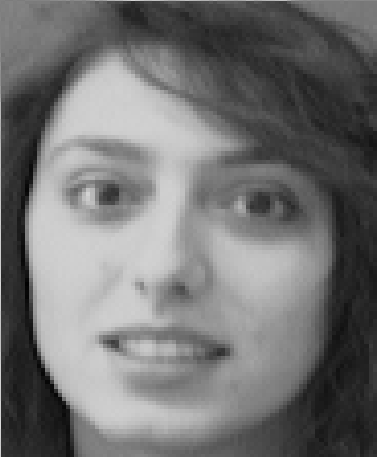
\includegraphics[scale=0.35]{img/1a_orig}
         \caption{Original image}
     \end{subfigure}%
     \quad
     \begin{subfigure}[t]{0.4\textwidth}
         \centering
         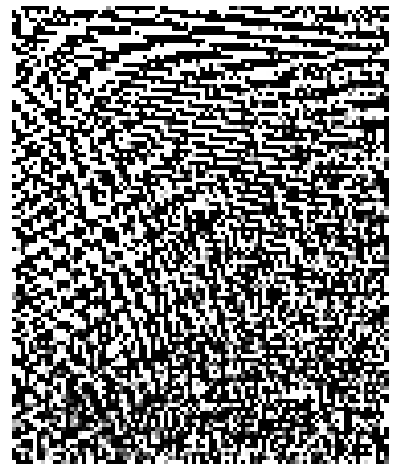
\includegraphics[scale=0.35]{img/1a_dct}
         \caption{DCT representation}
     \end{subfigure}
    \caption{Sample face image before and after applying DCT.}
    \label{fig:ex1a}
\end{figure}

\textbf{b)} \emph{Using the original configuration parameters (train = 6 images, test = 4 images, DCT coefficients = 10), plot the resulting DET image and indicate the resulting EER.}

The resulting DET curve is shown in Figure \ref{fig:ex1b}. The EER achieved, marked with a circle on the image, is $5.6891\%$. Recall that this value represents the point where the false acceptance rate and false rejection rate are equal.

\begin{figure}[h!]
  \centering
    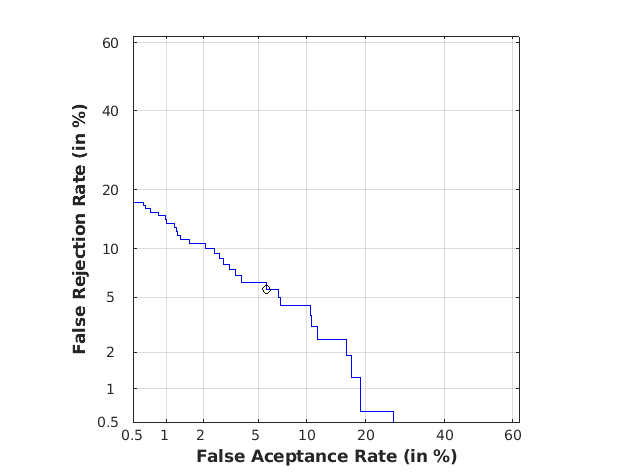
\includegraphics[scale=0.65]{img/1b_det}
    \caption{DET curve obtained with default parameters.}
    \label{fig:ex1b}
\end{figure}

\textbf{c)} \emph{Find out the configuration of the DCT coefficients that achieves the best EER results (keeping train = 6 images, test = 4 images). Justify your result, including the resulting DET image and EER value.}

Since we know that in general most images can be represented with just a few of the first DCT coefficients, we explore the best configuration in the search space in which the number of coefficientes varies from $1$ to $20$. The best EER result was $3.75\%$, obtained with \textit{coeff=5}, and the corresponding DET curve can be seen in Figure \ref{fig:ex1c}. We have achieved an EER that is about 2 percentage points smaller than the one obtained with the default parameters.

\begin{figure}[h!]
  \centering
    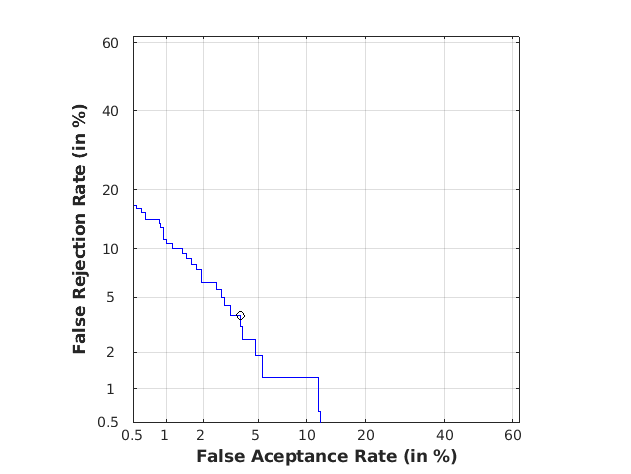
\includegraphics[scale=0.65]{img/1c_det}
    \caption{DET curve obtained with \textit{coeff=5}.}
    \label{fig:ex1c}
\end{figure}

Next we show in Figure \ref{fig:ex1c_bis} a comparison of the DET curves for all values \textit{coeff}$=1,\dots,20$, and also the evolution of the EER values with respect to the \textit{coeff} parameter.

\begin{figure}[h!]
  \centering
       \begin{subfigure}[t]{0.4\textwidth}
         \centering
         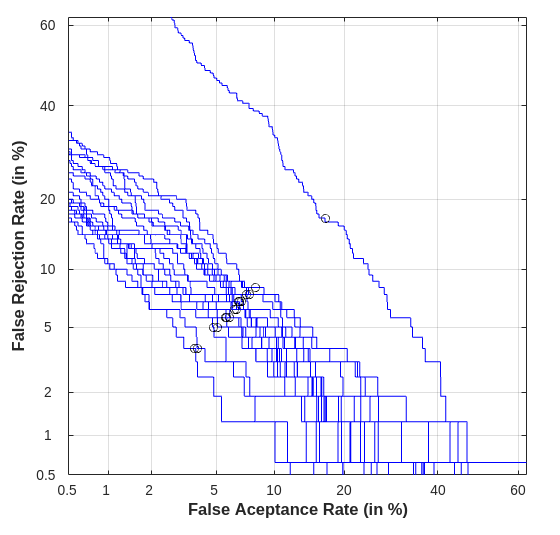
\includegraphics[scale=0.35]{img/1c_det_all}
         \caption{DET curves}
     \end{subfigure}%
     \quad \quad
     \begin{subfigure}[t]{0.4\textwidth}
         \centering
         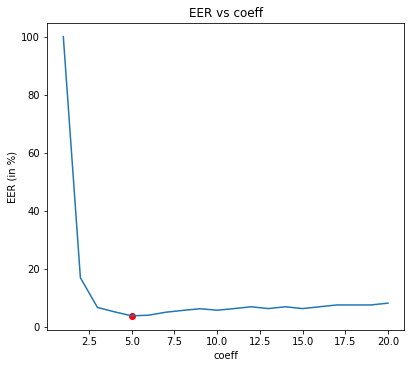
\includegraphics[scale=0.525]{img/1c_eer_evol}
         \caption{EER evolution}
     \end{subfigure}
    \caption{DET and EER for all values of \textit{coeff}.}
    \label{fig:ex1c_bis}
\end{figure}

\newpage
\textbf{d)} \textit{Once the best configuration of the DCT coefficients has been selected (in previous point), analyze the influence of the number of training images in the system performance. Include the EER result achieved for each case (from train = 1 to train = 7). Justify the results.}

We fix the parameter \textit{coeff}$=5$. Varying the value of \textit{train} from $1$ to $7$ (and setting \textit{test} to $10-$\textit{train}), the best EER result achieved was $3.3333\%$, obtained with \textit{train=7}, and the corresponding DET curve can be seen in Figure \ref{fig:ex1d}. As we can see, we have succeeded in lowering the EER obtained in \textbf{1c)}.

\begin{figure}[h!]
  \centering
    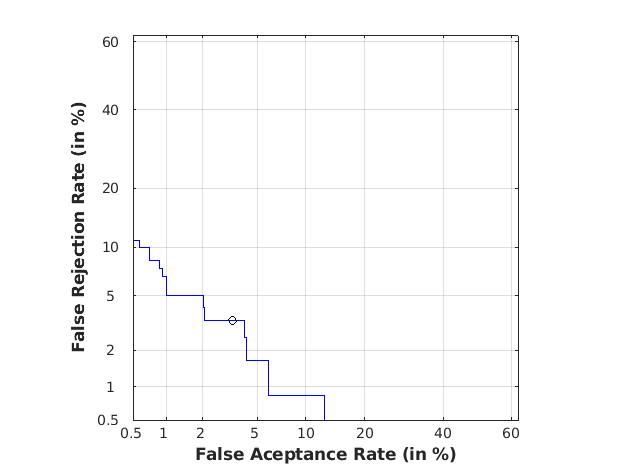
\includegraphics[scale=0.6]{img/1d_det}
    \caption{DET curve obtained with \textit{train=7}.}
    \label{fig:ex1d}
\end{figure}

The EER values obtained for each value of \textit{train} are summarized in Table \ref{tab:ex1d}, and a graph showing the evolution is shown in Figure \ref{fig:ex1d_bis}. The conclusion we draw is that a $70\%-30\%$ split in the dataset leads to better results regarding the EER.

\begin{table}[h!]
  \centering
  \begin{tabular}{c|ccccccc}
    \textbf{Train} & 1 & 2 & 3 & 4 & 5 & 6 & 7\\
    \hline
    \textbf{EER (\%)} & 13.0556 & 9.3750 & 6.4286 & 5.8333 & 5.0000 & 3.7500 & {\color{red}3.3333}
  \end{tabular}
  \caption{EER values obtained for each value of \textit{train}.}
  \label{tab:ex1d}
\end{table}

\begin{figure}[h!]
  \centering
    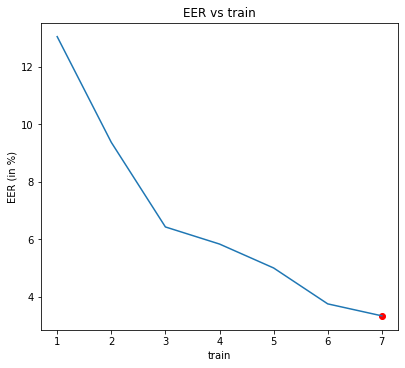
\includegraphics[scale=0.55]{img/1d_eer_evol}
    \caption{EER evolution for different values of the \textit{train} parameter.}
    \label{fig:ex1d_bis}
\end{figure}

\section*{Exercise 2}

\textit{The goal of this task is to change the feature extraction module. Instead of using DCT coefficients as in Task 1, you must consider \textbf{Principal Component Analysis (PCA)} to extract more robust features.}

The code implemented for this exercise can be seen in \verb|FaceRecognition_PCA.m|. The main ideas can be summarized as follows:

\begin{enumerate}
  \item Instead of performing feature extraction using DCT features, we want to use PCA features. For this purpose, we begin with the raw image matrices, and flatten them to a row vector. Next, we construct a matrix with all the training images (for every user) by vertically stacking the row vectors of each image, and we do the same for the test matrix.
  \begin{minted}{matlab}
% Convert image to row vector
im = reshape(im.', 1, []);

% Fill train matrix (i=user, j=image number)
MatrixTrainFeats((i-1)*Train + j, :) = im;
MatrixTrainLabels((i-1)*Train + j, 1) = i;
  \end{minted}
  \item We perform PCA on the newly constructed training matrix (using all images), and save the principal components, the projected training matrix, the variance explained by each principal component, and finally the mean vector of the columns of the original training matrix.
  \begin{minted}{matlab}
% Perform PCA with training values
[coeff_PCA,MatrixTrainPCAFeats,~,~,explained,mu] = ...
    pca(MatrixTrainFeats);
  \end{minted}
\item The last step before evaluating our model is to project the test features using the principal components. For this task, we need to first center the test matrix using the mean vector \verb|mu|, and then project (multiply) on \verb|coeff_PCA|.
\begin{minted}{matlab}
% Center and project test matrix on principal components
MatrixTestPCAFeats = (MatrixTestFeats - mu)*coeff_PCA;
\end{minted}
\end{enumerate}

\textbf{a)} \emph{Using the parameters train = 6 and test = 4, paste the DET curve and indicate the EER when using all the PCA components.}

The DET curve obtained is shown in Figure \ref{fig:ex2a}. We achieved an EER of $8.125\%$, which is worse than the results obtained with 10 DCT coefficients (default value in the previous exercise).

\begin{figure}[h!]
  \centering
    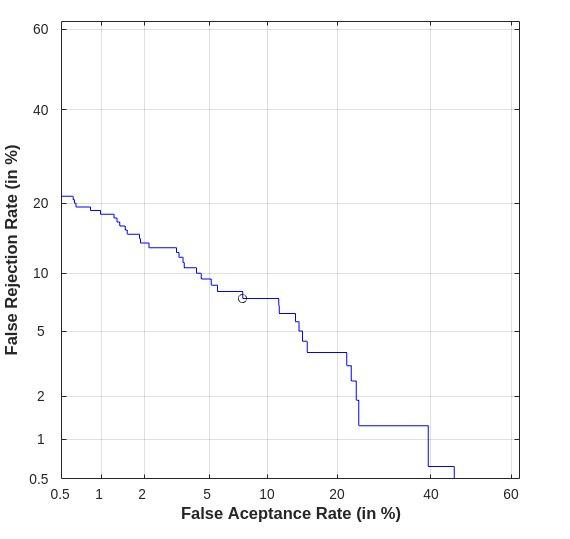
\includegraphics[scale=0.85]{img/2a_det}
    \caption{DET curve obtained using all PCA components.}
    \label{fig:ex2a}
\end{figure}

\textbf{b)} \emph{A key aspect for PCA is the number of components considered. Analyze and represent how the EER value changes in terms of the number of PCA components. Give your explanation about the results achieved.}

We can make the assumption that the result obtained in \textbf{a)} is not that good because we are using \textit{too many components} to represent our images. One might think that by retaining exactly the right amount of information, we could achieve a better result. With this idea in mind, we repeat the process above varying the number of principal components from $1$ to the maximum number available, which in this case is $239$, and we study the evolution of the EER achieved when considering $1,2,\dots,239$ principal components.

To project both the training and test matrices onto the first $L$ principal components, we do the following:
\begin{minted}{matlab}
MatrixTestPCAFeatsReduced = MatrixTestPCAFeats(:, 1:L);
MatrixTrainPCAFeatsReduced = MatrixTrainPCAFeats(:, 1:L);
\end{minted}

The graph mentioned above is shown in Figure \ref{fig:ex2b}, in which we see that after a certain number of components, the EER starts to increase, and then it tends to stabilize no matter how many components we consider. To try to explain this behaviour, we have also plotted the evolution of the $\%$ of variance explained by each of the principal components considered.

\begin{figure}[h!]
  \centering
       \begin{subfigure}[t]{0.4\textwidth}
         \centering
         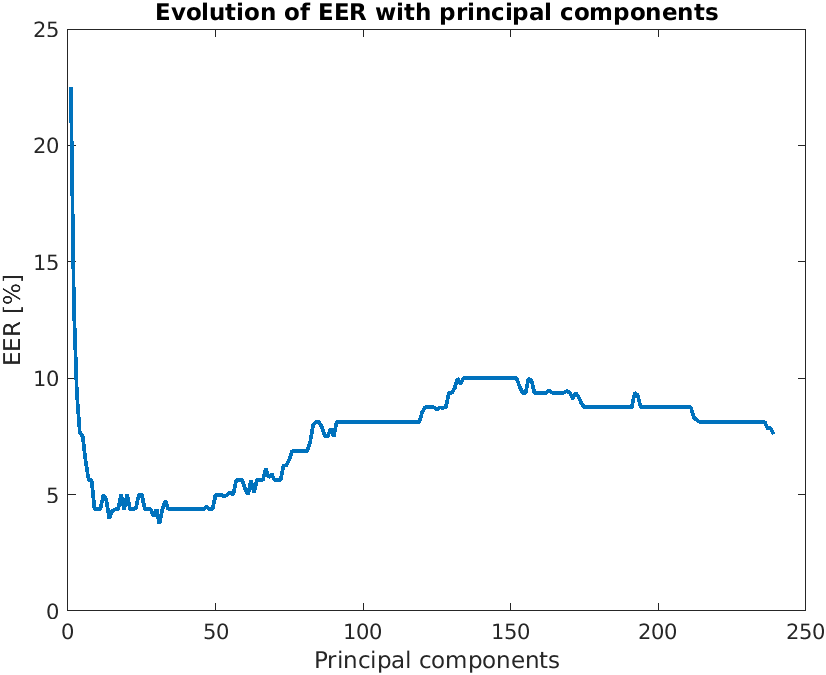
\includegraphics[scale=0.5]{img/2b_eer}
         \caption{EER}
     \end{subfigure}%
     \quad\quad
     \begin{subfigure}[t]{0.4\textwidth}
         \centering
         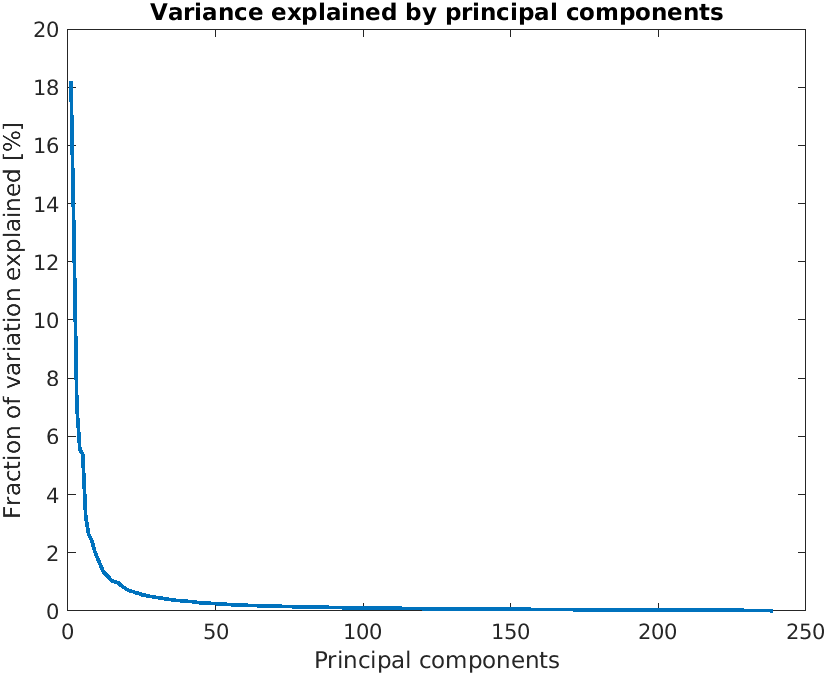
\includegraphics[scale=0.5]{img/2b_var}
         \caption{Variance explained}
     \end{subfigure}
    \caption{Evolution of EER and explained variance with the number of principal components.}
    \label{fig:ex2b}
\end{figure}

As we can see, at around 50 principal components the EER starts to increase, and it is precisely around that point where the $\%$ of explained variance that each new component contributes starts being negligible. We can conclude that we reach the optimal EER value by capturing the majority of explained variance, and stopping when the contributions drop below a reasonable threshold.

\textbf{c)} \textit{Indicate the optimal number of PCA components and paste the resulting DET curve together with the EER achieved. Compare the results using PCA with the DCT features considered in Task 1.}

The optimal number of PCA components found was $31$, reaching an EER value of $3.9103\%$ with a total explained variance of $78.2609\%$. The corresponding DET curve can be seen in Figure \ref{fig:ex2c}. This is almost the same value (only a bit worse) that we obtained in \textbf{1c)} with the optimal number of DCT coefficients (using the same number of training images), so we can say that both methods perform more or less equally well when doing feature extraction for the similarity measure, though not necessarily for other matching methods. However, the features extracted from PCA tend to be more robust and interpretable (in terms of the explained variance), so we prefer this latter approach.

\begin{figure}[h!]
  \centering
    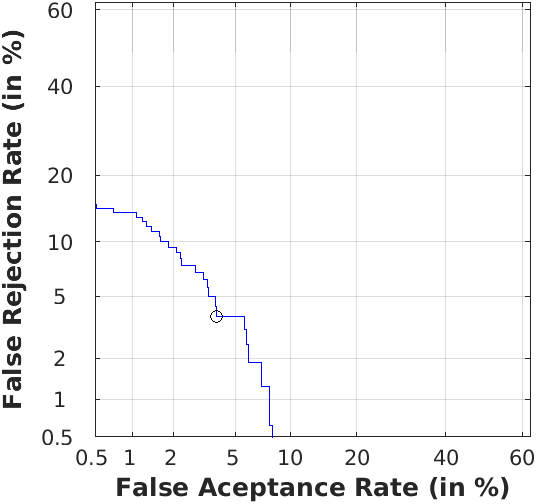
\includegraphics[scale=0.75]{img/2c_det}
    \caption{DET curve obtained using 31 PCA components (the optimal value).}
    \label{fig:ex2c}
\end{figure}

\section*{Exercise 3}

\textit{The goal of this task is to improve the matching module. Instead of using a simple distance comparison, you must consider Support Vector Machines (SVM). In this case, you should train one specific SVM model per user using the training data. Moreover, features extracted using the PCA module developed in Task 2 must be considered in this Task, using the parameters train = 6 and test = 4.}

The code implemented is available in the file \verb|FaceRecognition_SVM.m|. First of all, we consider the same PCA extraction module as in the previous exercise. Then, we train one SVM classifier per user with the \verb|fitcsvm| function, using their 6 training images as examples of the positive class, and all the training images of the rest of the users as negative examples:

\begin{minted}{matlab}
for i=1:n_users  % Train one classifier for each user
    labelsUser = MatrixTrainLabels == i;
    svmModel = fitcsvm(MatrixTrainPCAFeats, labelsUser);
    svms{i} = svmModel;
end
\end{minted}

Next, we evaluate each test image on each of the 40 classifiers, and use the scores to calculate the EER, as in the following code snippet:

\begin{minted}{matlab}
for i=1:n_users  % For each user
    % Predict using the SVM associated with user i
    [labelsSVM, scores]=predict(svms{i}, MatrixTestPCAFeats);

    % Fill Target or NonTarget depending on label coincidence
    maskUser = MatrixTestLabels(:, 1) == i;
    TargetScores=[TargetScores, scores(maskUser, 2)'];
    NonTargetScores=[NonTargetScores, scores(~maskUser, 2)'];
end
\end{minted}


\textbf{a)} \emph{Paste the DET curve and indicate the optimal EER found by varying the KernelFunction parameter of the SVM (using all PCA components).}

To change the kernel of each SVM we have to provide it with the parameter \verb|KernelFunction|. The first kernel tried was the linear kernel (by default), which can be expressed as $k(x, x')=x^Tx'$. Then we tried the polynomial kernel of degree 2, $k(x, x')=(x^Tx')^2$, and finally the RBF or Gaussian kernel, which is $k(x, x')=\exp(-\gamma\lVert x - x'\rVert^2)$, where $\gamma$ is a scale parameter. In this last kernel we set the \verb|KernelScale| parameter to \verb|'auto'| so that the software chooses the best value heuristically. The EER values achieved with each of the configurations can be seen in Table \ref{tab:ex3a}, while the corresponding DET curves are shown in Figure \ref{fig:ex3a}.

\begin{figure}[h!]
  \centering
       \begin{subfigure}[t]{0.4\textwidth}
         \centering
         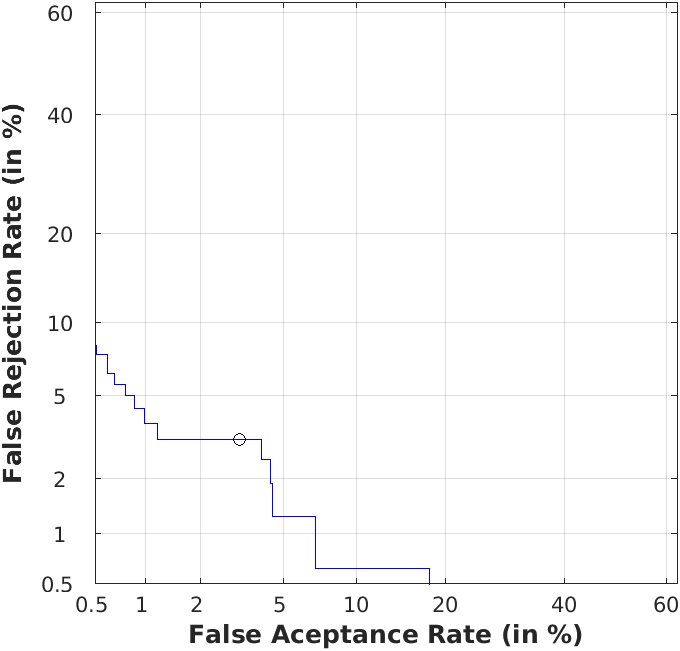
\includegraphics[scale=0.55]{img/3a_linear_det}
         \caption{Linear}
     \end{subfigure}%
     \quad\quad
     \begin{subfigure}[t]{0.4\textwidth}
         \centering
         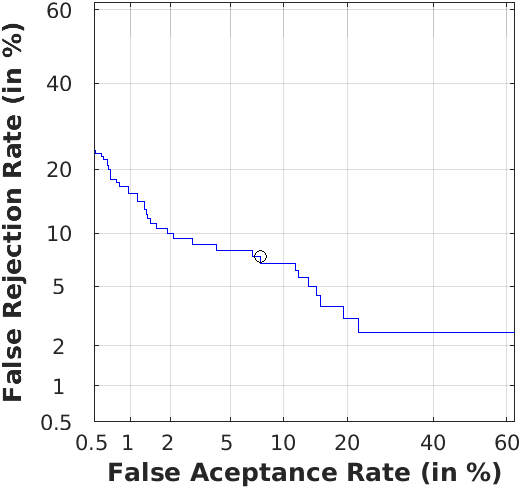
\includegraphics[scale=0.73]{img/3a_poly2_det}
         \caption{Polynomial degree 2}
     \end{subfigure}

     ~\vspace{1.5em}

     \begin{subfigure}[t]{0.4\textwidth}
         \centering
         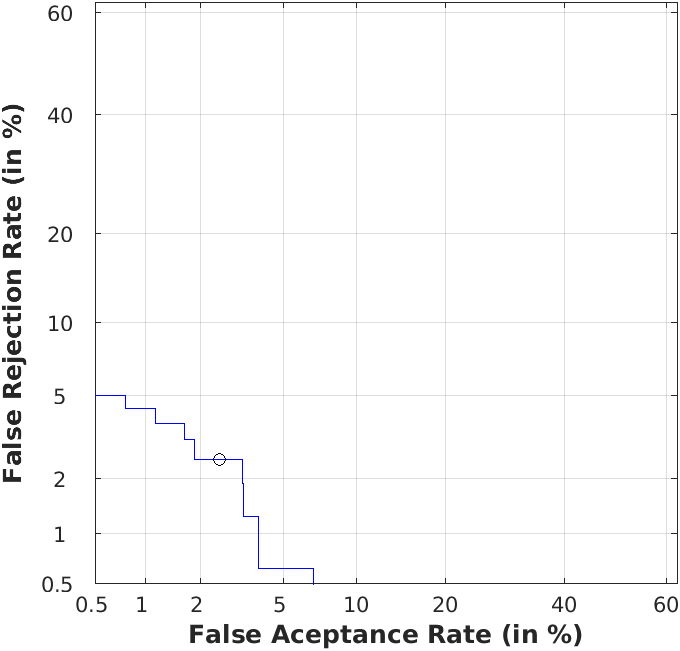
\includegraphics[scale=0.55]{img/3a_rbf_det}
         \caption{RBF + 'auto'}
     \end{subfigure}
    \caption{DET curves for each kernel choice using all PCA components.}
    \label{fig:ex3a}
\end{figure}

\begin{table}[h!]
  \centering
  \begin{tabular}{c|ccc}
    \textbf{Kernel} & Linear & Polynomial degree 2 & RBF + 'auto'\\
    \hline
    \textbf{EER (\%)} & 3.125 & 7.50 & {\color{red}2.5}\\
  \end{tabular}
  \caption{EER values obtained for each kernel choice using all PCA components.}
  \label{tab:ex3a}
\end{table}

As we can see, the best performing kernel is the RBF kernel, which is a well-known kernel that usually provides very good results. Next is the linear kernel, and even though it achieves a larger EER, this value is still lower than any EER obtained in the previous exercises. Finally, the polynomial kernel does not seem to perform well when using all 239 PCA components.

Note that exclusively for the polynomial kernel, we needed to standardize the data (centering and scaling) by setting the \verb|Standardize| parameter to \verb|true|, to reduce both computational time and the EER achieved. However, we did not standardize the data with the other kernels because the performance was poorer.

\textbf{b)} \textit{Paste the DET curve and indicate the optimal EER found by varying the number of PCA components considered for the feature extraction module (using the KernelFunction polynomial and starting with 3 PCA components).}

First of all, we fix the polynomial kernel of degree 2 (with standardized data), and let the number of PCA components used vary in $3,4,\dots, 239$. The optimal number of principal components found was 34, which resulted in an EER of $1.9391\%$. This is not a surprise, because 34 is quite close to the optimum number of PCA components found in the previous exercise for the similarity measure, and we saw that the explained variance started to decrease substantially not far from there. The curve that tracks EER evolution with respect to the number of components and the DET curve for the optimal value can be seen on Figure \ref{fig:ex3b_poly}.

\begin{figure}[h!]
  \centering
       \begin{subfigure}[t]{0.4\textwidth}
         \centering
         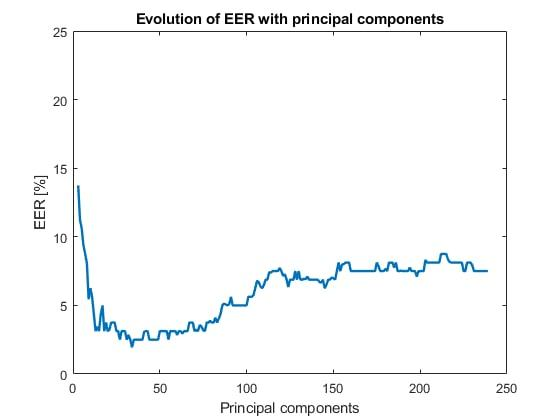
\includegraphics[scale=0.55]{img/3b_poly_eer}
         \caption{EER evolution}
     \end{subfigure}%
     \quad\quad
     \begin{subfigure}[t]{0.4\textwidth}
         \centering
         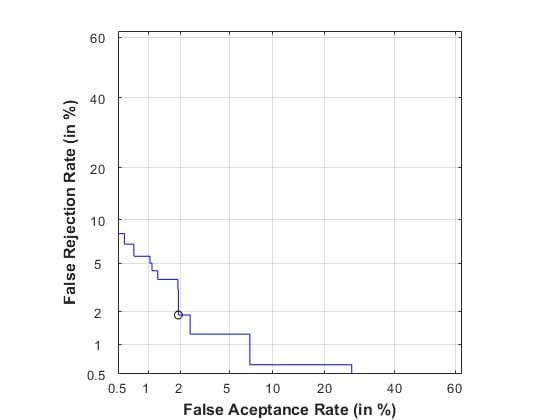
\includegraphics[scale=0.55]{img/3b_poly_det}
         \caption{DET curve for 34 components}
     \end{subfigure}
    \caption{EER evolution and optimal DET curve for the polynomial kernel.}
    \label{fig:ex3b_poly}
\end{figure}

As an added bonus\footnote{For this section we exploited Matlab's parallel capabilities, using \texttt{parloop} on the main cross-validation loop to distribute the code among several threads and speed up the computations.}, we repeated the process with the RBF kernel, to see which was the optimal number of PCA components in this case. We achieved an optimal EER of $1.8750\%$, the lowest we have seen, with just the first 12 principal components, which may seem a bit surprising. The evolution of the EER and the corresponding DET curve are shown in Figure \ref{fig:ex3b_rbf}.

\begin{figure}[h!]
  \centering
       \begin{subfigure}[t]{0.4\textwidth}
         \centering
         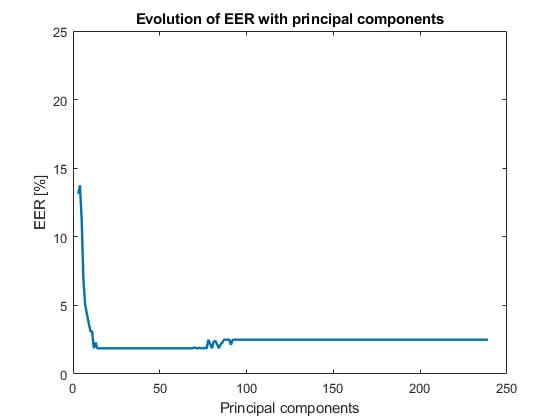
\includegraphics[scale=0.55]{img/3b_rbf_eer}
         \caption{EER evolution}
     \end{subfigure}%
     \quad\quad
     \begin{subfigure}[t]{0.4\textwidth}
         \centering
         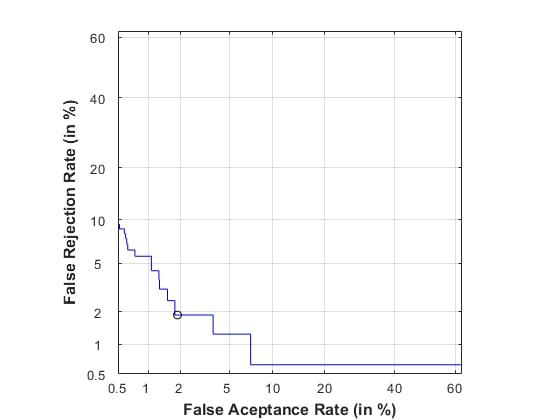
\includegraphics[scale=0.55]{img/3b_rbf_det}
         \caption{DET curve for 12 components}
     \end{subfigure}
    \caption{EER evolution and optimal DET curve for the RBF kernel.}
    \label{fig:ex3b_rbf}
\end{figure}

In conclusion, we have found that by carefully choosing a suitable number of PCA components and setting an appropriately tuned kernel function, we can decrease the EER to the lowest value seen so far, which is just below $2\%$. Since this value is quite low, we can confidently say that we expect the final classifier to have a very good performance.

\subsection*{A comment on the training examples}

In order to reduce execution time, we made some attempts at decreasing the number of negative examples that each SVM is trained on. We implemented the following code to select only \verb|n_train_extra| images from the rest of the users at random, where \verb|0 < n_train_extra < 235|:
\begin{minted}{matlab}
% Genuine class clabels
labels = [ones(Train, 1) ;
          zeros(n_train_extra, 1)];

% Get random training examples from other users
pop = [1:(i-1)*Train i*Train+1:n_users*Train];
random = randsample(pop, n_train_extra);

% Compute training matrix for user i
labelsUser = MatrixTrainLabels == i;
matrix = [MatrixTrainPCAFeats(labelsUser, :) ;
          MatrixTrainPCAFeats(random, :)];

% Train SVM
svmModel = fitcsvm(matrix, labels);
\end{minted}

We found that decreasing the number of negative training examples had a negative impact on the classification performance if we decreased the number too much, and for higher values the speedup was not substantial, so in the end we decided to stick with the whole training matrix. However, it is still possible that for a specific combination of some number of PCA components and a particular kernel, reducing the number of negative examples would increase the performance.

\subsection*{A comment on EER calculation}

While carrying out this assignment, we realized that the conventional EER definition for binary classifiers is not directly applicable here, as there is no such concept as a \textit{false positive} or a \textit{false negative} in a multi-class setting. Reviewing the literature in this regard, we found that in order to generalize the concept one may take different approaches, apart from the one pursued in this work. In particular, another common technique is to compute the EER of each of the One-vs-Rest classifiers and then compute some kind of weighted average. For example, \href{https://scikit-learn.org/stable/auto_examples/model_selection/plot_roc.html}{this is what sklearn does} when asked to compute the ROC curve or the AUC score (area below the ROC curve).

We thought about implementing this alternative metric calculation to compare it with the one we already use, but eventually we decided against it due to limited time and our lack of skill with Matlab. However, we do not rule out expanding on this line of work in the final project to compare different methods of EER calculation.

%TODO: repasar memoria, ejecutar todos los archivos una última vez.

\end{document}
